\section{An exact parameter for a Jordan crossing}\label{sec:crossing}

The repository's quantitative Jordan packet gives a particularly sharp
selection problem. For a path whose endpoints have different inside/outside
bits it constructs, for each precision, a close pair of path and curve
parameters. Its statement and its proof of approximate intersections explicitly
leave the selection of an exact crossing parameter open for general paths.%
\footnote{ProveIt, \href{https://github.com/VladimirReshetnikov/ProveIt/tree/5f3be02388442f16487d2dc5c2529961dd783d2b/Logic/PrimitiveRecursiveArithmetic/docs/proofs/topology/jordan_ipra_constructive_2026-11-15/sections}{Jordan packet, sections 1 and 4}.}
Close pairs chosen on unrelated meshes can alternate between different
crossings indefinitely. We give a local condition which makes the searches
coherent. An algebraic estimate supplies this condition even when the crossing
set has several points and a crossing has multiplicity greater than one.

\subsection{A bracket with a computable interior probe}

Write $\delta_j=2^{-j}$. Use the maximum norm on the plane and circular
distance $d_{\mathbb T}(u,v)=\min(|u-v|,1-|u-v|)$ on rational
representatives in $[0,1)$. Let $c:[0,1]\to\mathbb R^2$ be a presented
path and $g:\mathbb T\to\mathbb R^2$ a presented Jordan curve, both with
fixed PR rational evaluators of error $\delta_j$. Use nondecreasing PR
forward moduli $W,U$, respectively. Thus $|u-v|\le\delta_{W(j)}$
gives $\|c(u)-c(v)\|\le\delta_j$, and similarly for $g$. The Jordan
presentation also gives a nondecreasing PR inverse modulus (take the running
maximum if needed)
\[
 d_{\mathbb T}(u,v)\ge\delta_j
 \quad\Longrightarrow\quad \|g(u)-g(v)\|\ge\delta_{V(j)}.
\]
All inequalities about names can be read at rational stages, with the sum
of the two evaluation errors added to an upper bound or subtracted from
a lower bound. Bounds needed at later stages are computed by composition
of the moduli.

A mark $(t,k)$ records a rational time and a clearance exponent. There is a
finite Boolean test for such a mark. Evaluate $c(t)$ and the samples of $g$
at precision $k+4$ on a circle mesh of step $\delta_{U(k+4)}$.
Accept when the minimum of the rational sample distances exceeds
$\delta_k/2$. Clearance at least $\delta_k$ implies acceptance, since
the two evaluation errors cost at most $2\delta_k/16$. Acceptance implies
clearance greater than $\delta_k/4$, since these two errors and interpolation
from the mesh cost at most $3\delta_k/16$. Consequently the packet's bit
can be evaluated with exponent $k+2$. Give failed marks an arbitrary default
bit to obtain a total PR function. The inherited bit of a cleared point is independent of its mark. A subpath whose
cleared endpoints have different bits admits bounded approximate contact.
The latter algorithm is uniform in rational endpoints $a,b$, since
$u\mapsto c(a+(b-a)u)$ retains the forward modulus $W$ when $b-a\le1$.

\paragraph{Interior probe hypothesis.}
For every bracket $I=[a,b]\subseteq[0,1]$ with accepted, differently
labeled endpoints and $a<b$, a fixed PR routine supplies an accepted mark
$(p,k)$ with
\[
 a+(b-a)/4\le p\le b-(b-a)/4.
\]
This requires no designation of which intersection will be selected.
The initial bracket can be any such $I$.

\paragraph{Exact crossing theorem.}
From the initial bracket and the probe, fixed PR routines construct fast
parameter names $s_n\in[0,1]$, $t_n\in\mathbb T$ with
$c(s)=g(t)$ as an equality of completed names. One may retain an explicit
choice of intersection even if the initial bracket contains several.

\emph{Proof.}
Retain $[p,b]$ if the probe has the left bit and $[a,p]$ otherwise.
The new endpoints have opposite bits. The new width is between one quarter
and three quarters of the old width. Write $I_i$ for the bracket after $i$
cuts. Three cuts reduce the width by a factor at most $27/64<1/2$, so
$|I_{3r}|\le\delta_r$. For $n\ge0$ put
\[
 H(n)=4+\max(n,V(n+1)),\qquad
 K(n)=\max\{H(n),W(H(n))\}.
\]
On the subpath over $I_{3K(n)}$ find rational $s_n$ in that bracket and a
rational circular parameter $t_n$ with
$\|c(s_n)-g(t_n)\|<\delta_{H(n)}$. Concretely, take meshes whose
interpolation and evaluation errors together are at most $\delta_{H(n)}/8$
on each side and choose the first minimizing pair. If its measured distance
were at least $\delta_{H(n)}/2$, the entire subpath would have positive
clearance, contradicting the endpoint bits by the Jordan separation
interface. Otherwise the desired strict bound follows by adding the
evaluation errors. Thus this is bounded selection.

For $m\ge n$ both path parameters belong to $I_{3K(n)}$. Their difference
is at most $\delta_{K(n)}$ and the variation of $c$ is at most
$\delta_{H(n)}$. The triangle inequality gives
\[
 \|g(t_m)-g(t_n)\|<3\delta_{H(n)}<\delta_{V(n+1)}.
\]
Rational circular distance is decidable, so the inverse modulus gives
$d_{\mathbb T}(t_m,t_n)<\delta_{n+1}$. These are fast names for $s,t$.
For equality of images at requested error $\delta_j$, use an index at least
$\max(j+3,W(j+3),U(j+3))$. The two forward-modulus errors and the
middle contact error sum to less than $\delta_j$ (and rational evaluation can
be padded by two further bits). This constructs the two names directly.\hfill$\square$

\paragraph{A scalar version independent of the Jordan packet.}
For a scalar uniformly continuous presented $f$, assume opposite strict
signs at $a,b$. A probe with an explicit positive bound on $|f(p)|$
has a computable sign. The same cuts construct a fast name of a zero.
Indeed the values at the two ends of any retained interval straddle zero,
so the absolute value at either end is bounded by the oscillation there.
At depth $3\max(n,W(n))$ the left endpoint is within $\delta_n$ in time
of all subsequent endpoints and its residual is at most $\delta_n$.
This proof uses only the scalar sign and forward modulus. It also explains
why a probe guarantee is substantive. For $|z|\le1/4$ consider
\[
 f_z(t)=\min(3t-1,0)+\max(3t-2,0)+z .
\]
Every $f_z$ has opposite endpoint signs. For $z>0$ its only zero is
$(1-z)/3$. For $z<0$ the only zero is $(2-z)/3$. At $z=0$ there is an
interval of zeros. Any uniform finite-query routine on fast names must
produce its $1/16$-accurate output for the zero input from finitely many
answers. Choose positive and negative rational $z$ small enough that names
of both can return precisely those same zero answers at the queried
precisions and give the exact value at finer precisions. Their forced
outputs agree, yet their two roots are at least $1/3$ apart. This rules out
an unrestricted uniform root selector on these names. This obstruction concerns uniform finite queries to names. An individual
arithmetic presentation may admit its own explicit selector.

\subsection{Producing the probes from algebraic data}

Suppose $g(\mathbb T)$ lies in $P^{-1}(0)$ for a displayed rational
bivariate polynomial $P$. Supply a rational $B\ge1$ bounding both images
in $[-B,B]^2$. Along the path suppose $P(c(t))=Q(t)/D(t)$ with
$Q\in\mathbb Q[t]$ nonzero, $0<D(t)\le E$ on the interval, and $E$
a given positive rational. A polynomial path has $D=1$. For a rational
path the identity and denominator bounds are separate input certificates.
Only inclusion of the curve in the zero locus is needed.

Write $P=\sum c_{ij}X^iY^j$. A rational Lipschitz bound on the box is
\[
 L=1+\sum_{i+j>0}|c_{ij}|(i+j)B^{i+j-1}.
\]
To see this, telescope each monomial as a product of $i+j$ factors, changing
one input factor at a time. Each other factor is bounded by $B$. Therefore
a lower bound $\eta$ on $|Q(p)|$ gives clearance at least $\eta/(EL)$
from every curve point.

Let $d=\deg Q\ge1$ and $A$ be its leading coefficient. On a bracket
of width $w$ take the $d+1$ equally spaced points
\[
 p_j=a+w/4+jh,\qquad h=w/(2d),\qquad 0\le j\le d .
\]
The maximum sampled absolute value satisfies
\[
 \max_j |Q(p_j)|\ \ge\ \frac{d!\,|A|}{2^d}
                \left(\frac{w}{2d}\right)^d.                \tag{*}
\]
Indeed the forward difference $Q(X+h)-Q(X)$ has degree $d-1$ and
leading coefficient $dAh$, by the binomial expansion. Repeating exactly
$d$ times gives the constant $d!Ah^d$. Each signed difference of numbers of
absolute value at most $M$ is bounded by $2M$ in absolute value, so the last
entry in the difference triangle is bounded by $2^d$ times the largest
initial entry. This proves (*). Take the first maximizing $p_j$. For $d=0$
take the midpoint, with $|Q(p)|=|A|$.

For explicit running bounds let $w_0$ be the initial width. Choose $C$ with
\[
 2^{-C}\le \frac{d!\,|A|\, w_0^d}{EL\,2^d(2d)^d}.
\]
A positive rational $u/v$ with integer $u,v\ge1$ admits $C=v$.
At cut $i$, $w\ge 4^{-i}w_0$, so the exponent $C+2di$ suffices for the
mark. The exponent is linear in the depth even when crossings coalesce.
For the constant case take $2^{-C}\le |A|/(EL)$ instead.
The computation uses fixed iteration and rational comparison. Neither a
root separation bound nor a root multiplicity computation is required.

\paragraph{Three crossings of a smooth closed curve.}
With the unit circle as target, set
\[
 R(t)=(t-\tfrac14)(t-\tfrac12)^3(t-\tfrac34),\qquad
 c(t)=(1+R(t))\left(\frac{1-t^2}{1+t^2},\frac{2t}{1+t^2}\right).
\]
On $[0,1]$ we have $|R|\le(3/4)^2(1/2)^3=9/128$.
For $P=X^2+Y^2-1$, the path residual simplifies to the monic degree-ten
polynomial $R(2+R)$. Endpoints have opposite signs. The three crossing
times $1/4,1/2,3/4$ give distinct points on the unit circle. The middle
zero has order three. Indeed $2+R>0$ and the displayed factorization
identifies every zero. In this example sign detects the two components and
the quarter-circle chart in the formula supplies the curve parameter
directly. Parameterize the circle by four successive quarter turns of
the rational chart in parentheses, each on an interval of length $1/4$.
At a zero, the circle parameter is $s/4$. For an explicit path modulus,
$|R(u)-R(v)|\le5|u-v|$ by telescoping its five factors of magnitude
at most one. Cross multiplication in the chart gives an upper bound
$4|u-v|$ for its maximum-norm variation, so $c$ has Lipschitz bound $13$
and $W(j)=j+4$ works. The exact-arithmetic example performs 24 cuts from $[0,1]$ and
from three narrower brackets, checking the final difference and the width
estimate on every cut. The wide bracket retains $1/4$ and the narrower ones
retain all three crossings individually.

\begin{figure}[ht]
\centering
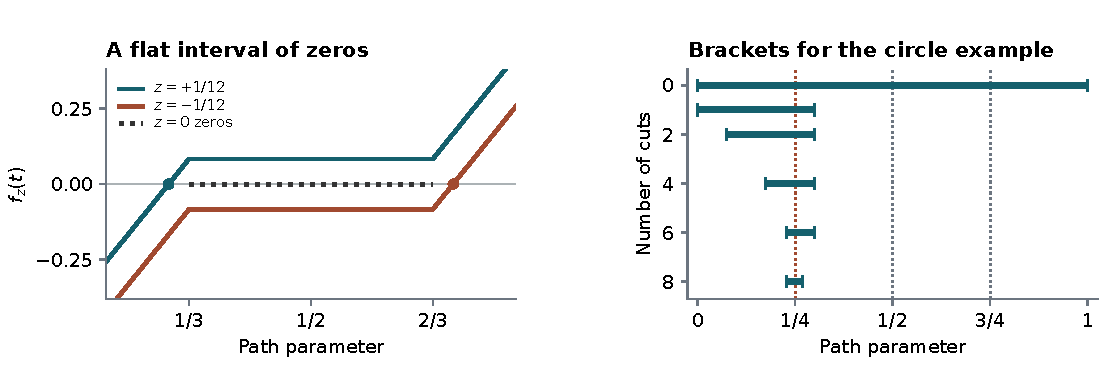
\includegraphics[width=0.97\linewidth]{figures/root_selection.pdf}
\caption{On the left the parameter \(z\) moves a flat segment through zero. The unique roots of the positive and negative perturbations approach different ends of the segment. On the right each horizontal line is the bracket actually retained by the polynomial probe for the unit-circle example. The vertical lines mark the three exact crossing times.}\label{fig:crossings}
\end{figure}

\paragraph{Arithmetic and Lean implementation.}
A bracket stores two rational times and two integer clearance exponents.
After fixing the presentation, acceptance, bit, center-quarter tests and
the cut are PR. The loop invariant is the conjunction of rational ordering,
two accepted marks, opposite bits, nestedness relative to a frozen starting
bracket, and rational width bounds. Each is a Boolean test after coding.
The analytic soundness of the acceptance test is used on demand outside
this induction. For the difference triangle, rational evaluations, maxima
and the entire triangular table have PR codes. Fix its input table and
degree before induction on the row. The invariant is a bounded conjunction
of the row-entry enclosures, encoded by a single PR bit. Similarly polynomial
difference identities follow by coefficient comparison with finite sums for
the binomial expansion. Fixing the modulus query before each width or
triangle induction suffices for quantifier-free induction.

The module \texttt{TopologyCase.lean} proves the bracket step, iteration
invariant, three-step estimate, rate $2^n w_{3n}\le w_0$, and both ingredients of (*) in Lean over rational numbers.
Its \texttt{horner\_top\_difference} proves the exact $d$th difference
identity for every coefficient list and arithmetic progression, and
\texttt{polynomial\_probe\_bound} combines that identity with the signed
enclosure of the difference triangle.

There is also an object derivation for the polynomial identity itself.
In \texttt{TopologyObject.lean}, \texttt{CrossingObject.top\_difference}
constructs a \texttt{Prf PRAAx} of the signed integer equation for every
externally fixed degree and arbitrary integer terms for the coefficients,
origin and step. It interprets the difference fold and Horner evaluation in
the ring of differences of the iPRA term model, proves the identity there,
and applies the repository's \texttt{ZT.derive}. For rational inputs take
a positive common denominator $B_0$, write $x=X/B_0$, $h=H_0/B_0$ and the
coefficients as $b_j/B_0$. Multiplying by $B_0^{d+1}$ turns the sampled
polynomial into $\sum_{j=0}^d b_j B_0^{d-j}(X+iH_0)^j$ at sample $i$.
This directly specifies the signed integer instance to use. Transport back
amounts to cancellation of the positive denominator. The object file
produces the signed polynomial equation. Rational clearing and the
enclosure inequality still need object proofs.

To complete the bracket derivations,
instantiate rational comparisons by cross multiplication on positive
denominators, lift addition and multiplication of signed pairs, and
use these identities for each branch of \texttt{cut\_spec}. Apply
quantifier-free induction to the compiled good-state bit to obtain the
iteration lemma and twice to the width and difference folds. The remaining
analytic interfaces for a general Jordan input are the bit's
positive-clearance stability, the forward and inverse moduli, and the
evaluator error estimates. The packet supplies human arguments for the
Jordan interface. The object derivations still to be constructed cover this
Jordan interface, the rational inequalities and the specialized bracket
inductions.
